
	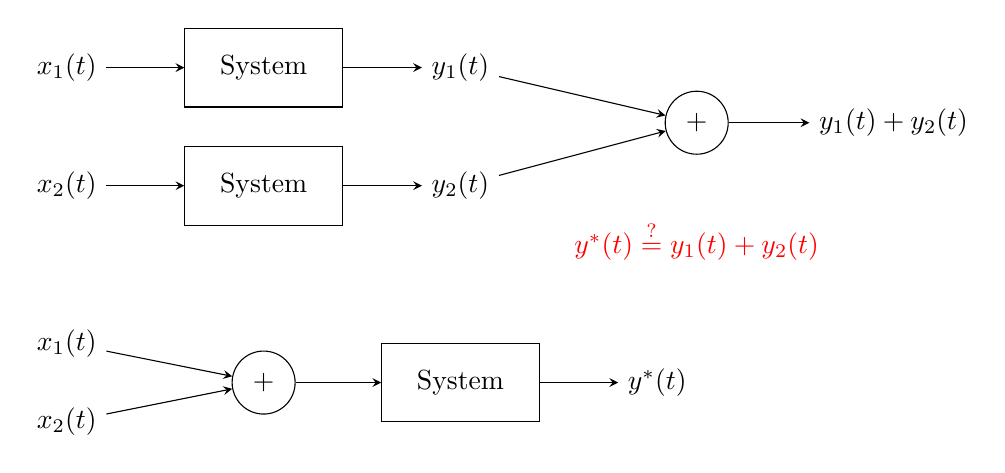
\begin{tikzpicture}[
		block/.style={rectangle, draw, minimum width=2cm, minimum height=1cm, align=center},
		sum/.style={circle, draw, minimum size=0.8cm, align=center},
		node distance=2.5cm,
		>=stealth
		]
		
		% Top row - Individual systems
		% First path: x1(t) -> System -> y1(t)
		\node (x1) {$x_1(t)$};
		\node[block, right of=x1] (sys1) {System};
		\node[right of=sys1] (y1) {$y_1(t)$};
		
		% Second path: x2(t) -> System -> y2(t)  
		\node[below of=x1, node distance=1.5cm] (x2) {$x_2(t)$};
		\node[block, right of=x2] (sys2) {System};
		\node[right of=sys2] (y2) {$y_2(t)$};
		
		% Bottom row - Combined system
		% Input summing junction
		\node[below of=x2, node distance=2cm] (x1_bottom) {$x_1(t)$};
		\node[below of=x1_bottom, node distance=1cm] (x2_bottom) {$x_2(t)$};
		\node[sum, right of=x1_bottom, yshift=-0.5cm] (sum_input) {$+$};
		\node[block, right of=sum_input] (sys_combined) {System};
		\node[right of=sys_combined] (y_prime) {$y^*(t)$};
		
		% Right side - Comparison and output summing
		\node[sum, right of=y1, node distance=3cm,yshift=-0.7cm] (sum_output) {$+$};
		\node[right of=sum_output] (sum_result) {$y_1(t) + y_2(t)$};
		
		% Comparison question
		\node[below of=sum_output, node distance=1.5cm , red] (comparison) {$y^*(t) \stackrel{?}{=} y_1(t) + y_2(t)$};
		
		% Arrows for top row
		\draw[->] (x1) -- (sys1);
		\draw[->] (sys1) -- (y1);
		\draw[->] (x2) -- (sys2);
		\draw[->] (sys2) -- (y2);
		
		% Arrows for bottom row
		\draw[->] (x1_bottom) -- (sum_input);
		\draw[->] (x2_bottom) -- (sum_input);
		\draw[->] (sum_input) -- (sys_combined);
		\draw[->] (sys_combined) -- (y_prime);
		
		% Arrows for output summing
		\draw[->] (y1) -- (sum_output);
		\draw[->] (y2) -- (sum_output);
		\draw[->] (sum_output) -- (sum_result);
		
		
	\end{tikzpicture}

